\newcommand{\ion}{HC$_3$N$^+$}
\newcommand{\neion}{Ne$-$\ion}
\newcommand{\iont}{HC$_3$N$^+$ ion}
% \newcommand{\wn}{cm$^{-1}$}
\newcommand{\wns}{cm$^{-1}$ }
\newcommand{\bmH}{\bm H}
\newcommand{\bmn}{\bm n}
\newcommand{\bra}[1]{\langle #1 |}
\newcommand{\ket}[1]{| #1 \rangle}
\newcommand{\braket}[2]{\langle #1 | #2 \rangle}

% \draft % marks overfull lines with a black rule on the right

\section*{Abstract}
The linear radical cation of cyanoacetylene, \ion ($^2\Pi$), is not only of astrophysical interest, being the, so far undetected, cationic counterpart of the abundant cyanoaceteylene, but is also of fundamental spectroscopic interest due to its strong spin-orbit and Renner-Teller interactions. Here, we present the first broadband vibrational action spectroscopic investigation of this ion through the infrared pre-dissociation (IRPD) method using a Ne tag. Experiments have been performed using the FELion cryogenic ion-trap instrument in combination with the FELIX free-electron lasers and a Laservision OPO/OPA system. The vibronic splitting patterns of the three interacting bending modes ($\nu_5$,$\nu_6$, $\nu_7$), ranging from $180-1600$~\wn, could be fully resolved revealing several bands that were previously unobserved. The associated Renner-Teller and intermode coupling constants have been determined by fitting an effective Hamiltonian to the experimental data, and the obtained spectroscopic constants are in reasonable agreement with previous photoelectron spectroscopy (PES) studies and \emph{ab initio} calculations on the \ion\ ion. The influence of the attached Ne atom on the infrared spectrum has been investigated by \emph{ab initio} calculations at the RCCSD(T)-F12a level of theory, which strongly indicates that the discrepancies between the IRPD and PES data are a result of the effects of the Ne attachment.
\clearpage
% \pacs{}% insert suggested PACS numbers in braces on next line

\section{Introduction}
The simplest cyanopolyyne,  cyanoacetylene (HC$_3$N), is one of the most wide-spread polyatomic species in the interstellar medium (ISM) and has been observed in a variety of astronomical sources in the Milky Way and in external galaxies\cite{Turner1971DetectionCyanoacetylene,Morris1976CyanoacetleneClouds, Mauersberger1990DenseProbe}. 
It also plays an important role in the complex nitrogen chemistry of Titan, Saturn's largest moon, being one of the most abundant nitrogen bearing species detected in its atmosphere. \cite{Cordiner2014ALMAAtmosphere,Thelen2019AbundanceObservations}.
Its highly reactive cationic counterpart, \ion, is efficiently produced by ionization of the neutral cyanoacetylene by solar vacuum-ultraviolet (VUV) radiation and may participate in Titan's thiolin formation \cite{VYA2006}.
In the ISM, neutral HC$_3$N is readily ionized by cosmic rays or UV photons to form \ion \cite{Wakelam2012AKIDA}.  However, this cation has yet to be detected in the ISM, which is likely a result of lack of reference data.

Besides being astrochemically relevant, the cyanoacetylene radical cation ($ ^2\Pi$) is interesting on a fundamental spectroscopic level due its open-shell linear character. 
The vibronic coupling effects that occur as a result of this character, such as Renner-Teller (RT) \cite{RennerZurMolekiilen} coupling, cause a breakdown of the Born-Oppenheimer (BO) approximation. 
Subsequent analysis of the complex splitting pattern then requires methods that go beyond the BO approximation, such as effective Hamiltonian analysis (for small couplings)\cite{He2005} or a full nonadiabatic description of the molecule.\cite{Peric2007AMolecule,Koppel1981VibronicStates}

Previous work on \ion\ includes several low- and high-resolution photoelectron spectroscopy (PES) studies \cite{Dai2015TheCalculations,Desrier2016ExperimentalSpectroscopy,Gans2016ExperimentalSpectroscopy,Leach2014IonizationCyanoacetylene}. The high-resolution pulsed-field ionization zero kinetic energy (PFI-ZEKE) study by  \citet{Dai2015TheCalculations} presented sufficient experimental resolution to reveal an intricate RT and spin-orbit (SO) splitting pattern in the observed vibronic spectrum, which was analyzed on the basis of diabatic calculations. 
The observed medium to weak coupling strengths make this ion an excellent candidate for an effective Hamiltonian analysis rendering experimental spectroscopic constants that can be used to benchmark \emph{ab initio} calculations.

Vibrational spectroscopic work on \ion\ is limited to a Ne-matrix assisted absorption spectroscopy study in the C-H stretching region\cite{Smith-Gicklhorn2001VibrationalCations}, which does not contain any information on the three RT affected vibrational bending modes. Gaining information on these modes through vibrational spectroscopy would be complementary to the earlier PES work due to the different selection rules at hand and would aid to a full understanding of this complex ion. Furthermore, this data could serve as a reference for future high-resolution studies and for astronomical searches (e.g., with the James Webb Space Telescope operating in the infrared region).

Infrared pre-dissociation spectroscopy (IRPD) is an excellent method to obtain gas-phase vibrational spectra of molecular ions. Here a messenger (usually a rare-gas atom) is weakly bound to the target ion at cryogenic temperatures and its subsequent on-resonant dissociation is monitored by mass spectrometry. This messenger atom, also called tag, acts as a spectator and in the case of rare-gas atoms like He or Ne its influence on the vibrational structure is generally rather small \cite{Marimuthu2020LaboratorySpectroscopy, Marimuthu2021InfraredCH3CNH+, Rap2020StableSpectroscopy}.   
This method is especially suited for small reactive cations, since other (tag-free) action spectroscopic methods are not suitable \cite{Roithovareview}(e.g.infrared multi-photon dissociation is limited due to the small size of the ion \cite{Jasikova2018,Brodbelt2009}, laser induced reactions \cite{schlemmer_laser_2002} require a suitable endothermic reaction,  and laser inhibition of complex growth \cite{Chakrabarty2013, Asvany2015} does work only with cw lasers). 

The goal of the present study is to obtain the first broad-band gas-phase vibrational spectrum of the \ion\ cation covering all fundamental vibrational modes including the RT perturbed bending modes, in order to complement and extend  the earlier PES studies. 
The spectrum was recorded by means of infrared pre-dissociation spectroscopy (IRPD) using Ne as a rare-gas (RG) messenger atom carried out in a cryogenic ion trap interfaced with the widely tunable FELIX (Free Electron Laser for Infrared eXperiments) \cite{oepts_free-electron-laser_1995} free electron laser \cite{jusko_felion_2019}. 
The recorded spectrum is fitted with an effective Hamiltonian and compared to \emph{ab initio} calculation of \citet{Dai2015TheCalculations}, and the results are discussed with an emphasis on the influence of the Ne atom used as a tag in the IRPD scheme.


\section{Methods}
\subsection{Experimental methods}
\label{sec:experiment}
The vibrational spectrum of the cyanoacetylene cation (\ion) was recorded using the FELion cryogenic 22-pole ion trap instrument. A detailed account of the FELion instrument is provided in Section \ref{sec:felion} and the infrared-predissociation (IRPD) of in-situ rare gas tagged cold molecular ions in Section \ref{subsec:action:methods:vibrational:IRPD}, and here we only give a brief account of details specific to the \iont. The ion is produced by direct electron impact ionization [$28(2)$~eV] from the neutral precursor acrylonitrile (CH$_2$CHCN, $ \ge 99\%$ purity, Sigma-Aldrich). The liquid precursor was evaporated into the ion source and diluted with helium in a 5:1 (He:CH$_2$CHCN) mixing ratio. An about 100~ms long pulse of ions is extracted from the source and the ions of interest, {\em i.e.},\ \ion\ with m/z 51, are mass selected by a quadrupole mass filter before entering the 22-pole ion trap which is held at a fixed temperature in the range $8-9$~K.  Around $10-15$~ms before the ions enter the trap, an intense $\sim$80~ms long Ne:He pulse (1:3 mixing ratio and number density of $\sim 10^{15}$~cm$^{-3}$) is admitted to the trap, leading to efficient collisional cooling of the ions close to the trap ambient temperature and the formation of Ne-ion complexes by termolecular collisions. Under these conditions, around $\sim 10 \%$ of the primary ions form weakly bound complexes with Ne, see Fig.~\ref{fig:HC3N+masspec}.

\begin{figure}[tb]
    \centering
     \begin{subfigure}[b]{0.48\textwidth}
         \centering
         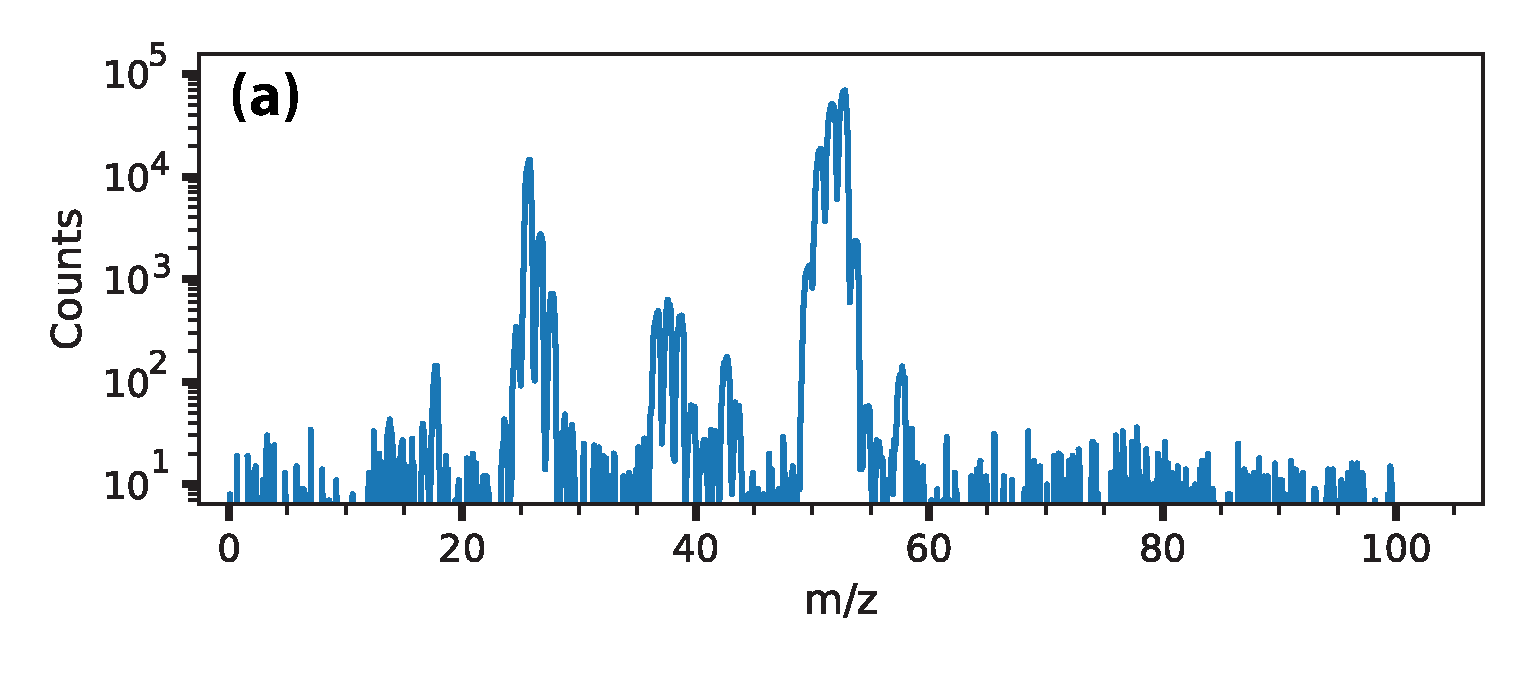
\includegraphics[width=1\textwidth]{chapters/HC3N+/figures/masspec/modified/HC3N+_masspec.eps}
        %  \caption{}
         \label{fig:HC3N+masspec:background}
     \end{subfigure}
     \hfill
     \begin{subfigure}[b]{0.49\textwidth}
         \centering
         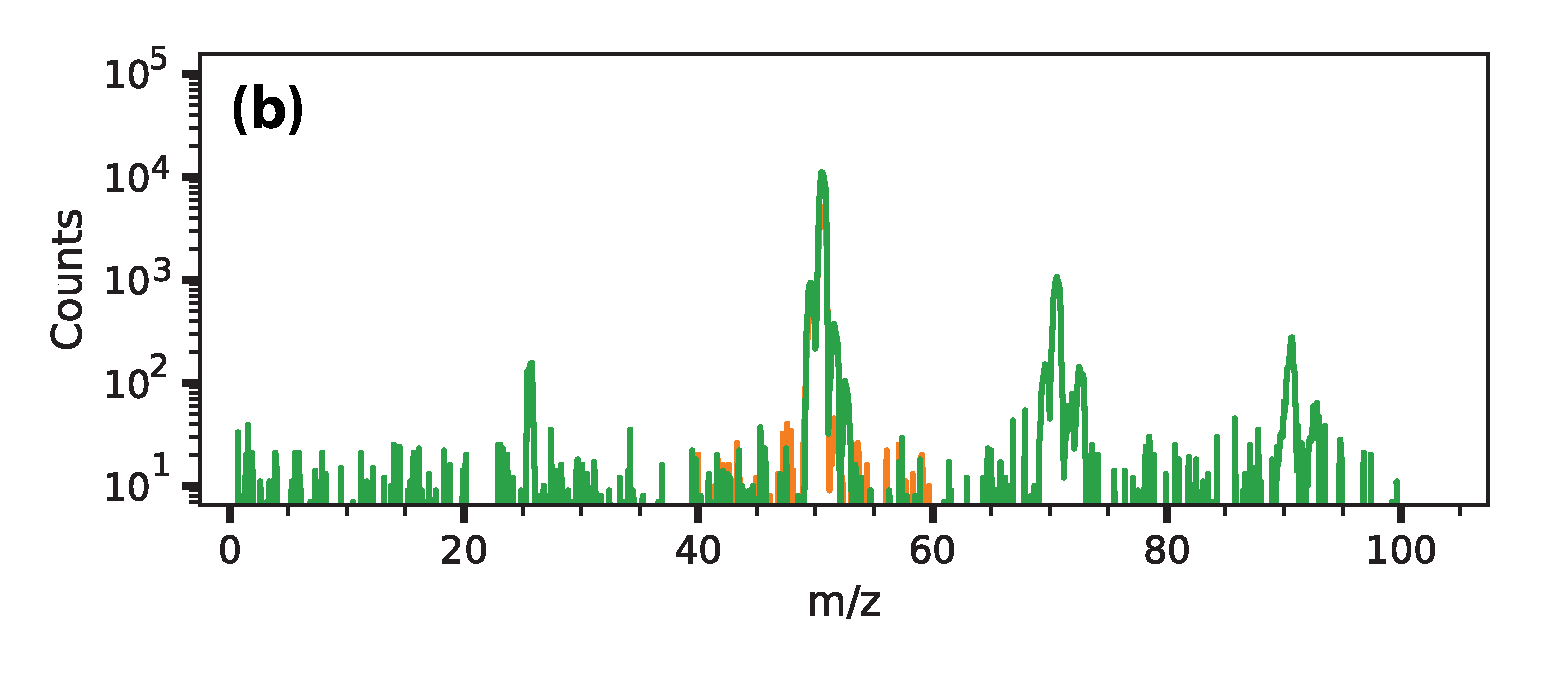
\includegraphics[width=1\textwidth]{chapters/HC3N+/figures/masspec/modified/HC3N+_masspec_complex.eps}
        %  \caption{}
         \label{fig:HC3N+masspec:complex}
     \end{subfigure}
    \caption{(a) Mass spectrum of ions produced from electron impact ionization ($\sim 28$~eV) of acrylonitrile (blue). (b) Mass-selected (orange) \ion\ (m/z  51) together with tagged (green) \neion\ (m/z  71) complexes produced in the cryogenic ion trap at temperature 8.5(2)~K and He:Ne gas mixture number density of 9(1)$\cdot 10^{14}$~cm$^{-3}$. The attachment of isotopic $^{22}$Ne can also be seen in panel (b).  A small contamination from C$_3$N$^+$ (m/z 50) can be seen in the mass-selected spectrum, resulting from insufficient mass-filtering of the primary ions.}
    \label{fig:HC3N+masspec}
\end{figure}

The ions are stored for several seconds in the ion trap (typically $1-3$~s) and are exposed to several FELIX IR laser pulses before extraction. An IRPD spectrum is recorded by mass-selecting and detecting the \neion\ complex ions as a function of wavenumber. The following wavenumber ranges were covered in this study: (a) $130 - 270$~\wn, (b) $310 - 2500$~\wns, and (c) $3110 - 3270$~\wn, using the free-electron IR lasers FEL-1 (a) and FEL-2 (b) of the FELIX Laboratory\footnote{\url{https://www.ru.nl/felix/about-felix/about-felix/felix-laboratory/}} with macropulse repetition rate of 10~Hz, maximum pulse energy in the trap region of $< 35$~mJ (at 1100 \wn), and linewidths (fwhm) of around 0.5 \% of the center wavenumber.  Region (c) was covered using a Laservision OPO/OPA system ($\sim 1$~\wns  fwhm, 10 Hz repetition rate) with typical output power of $<20$~mJ. 

A relative depletion $D=1-\frac{N_\mathrm{ON}(\nu)}{N_\mathrm{OFF}}$ in the number of complex ions $N_\mathrm{ON}(\nu)$ from the baseline value $N_\mathrm{OFF}$ is observed upon resonant vibrational excitation. To account for varying laser pulse energy $E$, pulse number $n$, and for saturation effects, the signal is normalized prior to averaging using $I=\frac{-\ln[N_\mathrm{ON}(\nu)/N_\mathrm{OFF}]}{E(\text{in J})}$, giving the intensity $I$ in units of cross-section per Joule. After normalizing each individual spectrum in this way, the final spectrum is then obtained by averaging using statistical binning with a typical bin size of 2~\wn. Line parameters such as band positions, intensities, and line widths (fwhm) are then obtained by fitting a multi-component Gaussian function to the experimental data, also providing statistical errors of the line parameters.

\subsection{Theoretical approach}

\subsubsection{Ab Initio}
To understand and describe the vibrational IRPD spectra and the influence of the attached Ne atom on the observed band positions we performed \emph{ab initio} quantum chemical calculations on the \ion\ cation and the \neion\ complex. 
Geometry optimization and subsequent harmonic wavenumber calculations on the bare ion were performed at the partially spin-restricted, explicitly correlated, coupled cluster level of theory, with single, double, and perturbative triple excitations, RCCSD(T)-F12a \cite{Kong2012ExplicitlyStructure} using cc-pVXZ-F12 (X=D,T,Q) \cite{Peterson2008SystematicallyIN} basis sets, and for the \neion\ using the cc-pVTZ-F12 basis set. 
Information on the perpendicular component of the dipole moment of the bare ion was obtained by the use of finite-field perturbation theory, where a finite dipole field ($F=0.005$~a.u.) is added to the core energy and the one-electron Hamiltonian. The dipole moment $\mu$ is then obtained as
\begin{equation}
\label{eq:dipole}
    \mu=-\frac{E(+F) - E(-F)}{2F},
\end{equation}
where $E(F)$ is the energy as a function of the field.

To investigate the interaction of \ion\ with the Ne atom a one-dimensional cut of the potential energy surface was made by attaching the Ne atom to the middle carbon atom for fixed Ne-C-H angles, while optimizing all other geometry parameters. 
All quantum chemical calculations were performed using the MOLPRO suite, version 2015.1.\cite{Werner2020ThePackage}

\subsubsection{Effective Hamiltonian}
The spin-vibronic energy levels of HC$_3$N$^+$ were calculated with an effective Hamiltonian approach similar to the model of \citet{He2005} following the nomenclature employed by \citet{Dai2015TheCalculations}.
We ignore the effects of molecular rotation since its effects are too small to be seen with the experimental resolution of approximately 0.5\% of the center wavenumber: for \neion\ complex $B_e \approx $  0.033 \wn, calculated at the RCCSD(T)-F12a/cc-pVTZ-F12 level of theory. 

A Hund's case (a) basis, $\ket{\bm n}$, was chosen with: 
\begin{equation}
    \ket{\bm n} = |\Lambda \rangle |\Sigma \rangle \prod_{k=5}^7 |v_k, l_k \rangle |K \rangle |P \rangle.
    \label{eqn:Basis}
\end{equation}
Here, quantum numbers $\Lambda=\pm 1$ and $\Sigma=\pm 1/2$ are the projection of the orbital and spin angular momenta on the molecular axis, respectively, $v_k=0, 1, \dots$ is the vibrational quantum number of mode $v_k$ and $l_k$ is the projection of the vibrational angular momentum ($l_k=-v_k,-v_k+2,\ldots,v_k$).
We only include the three bend normal modes $v_5-v_7$.
Quantum number $K=\Lambda+\sum_k l_k$ is the projection of the total angular momentum excluding electron spin and $P=K+\Sigma$ is the projection of the total angular momentum onto the molecular axis.
In the case of strong vibronic coupling, such as RT coupling, $\Lambda$ and $l_k$ are ill-defined, but $P$ is a good quantum number since we neglect overall rotation. Furthermore, we only include diagonal spin-orbit coupling and first order RT, see below, and hence $K$ is also a good quantum number.
For a basis truncated at $v_\mathrm{tot}=v_5+v_6+v_7=8$ we find that energy levels are converged up to $v_\mathrm{tot}=3$.

We approximate the total effective Hamiltonian by: 
\begin{equation}
  \hat{H}=\hat{H}_\mathrm{vib} + \hat{H}_\mathrm{SO} + \hat{H}_\mathrm{RT}
    \label{eqn:Hamil},
\end{equation}
where $\hat{H}_\mathrm{vib}$ represents the harmonic vibrational energy,
\begin{equation}
  \hat{H}_\mathrm{vib} = \sum_{k=5}^7 \omega_k(\nu_k+1)\; |\nu_k\rangle \langle \nu_k|,    
\end{equation}
with $\omega_k$ the harmonic frequencies of the bending modes $\nu_5-\nu_7$. The spin-orbit Hamiltonian is given by \cite{Pople1960}
\begin{equation}
  \hat{H}_\mathrm{SO} = A_\mathrm{SO} \hat{L}_z \hat{S}_z,
\end{equation}
where we take the SO constant $A_\mathrm{SO}=-44$ cm$^{-1}$ independent of the vibrational mode \cite{Dai2015TheCalculations} and $\hat{L}_z$ and $\hat{S}_z$ are the molecule fixed components of the electronic orbital and spin angular momenta operators, respectively. The effective RT Hamiltonian is \cite{Brown1977TheEffect} 
%\begin{align}
%  \lefteqn{\hat{H}_\mathrm{RT} = \sum_{k=5}^7 %[\frac{1}{2}\epsilon_k\omega_k\{q_{k,+}^2\exp(-2i\theta)+q_{k,-}^2\exp(2i\theta %)\}]}\nonumber\\
%  &\mbox{} + \epsilon_{56}\sqrt{\omega_5\omega_6}\{q_{5,+}q_{6,+}\exp(-2i\theta)%+q_{5,-}q_{6,-}\exp(2i\theta)\}\\
%  &\mbox{}+ \epsilon_{57}\sqrt{\omega_5\omega_7}\{q_{5,+}q_{7,+}\exp(-2i\theta)+%q_{5,-}q_{7,-}\exp(2i\theta)\}\nonumber\\
%  &\mbox{} + \epsilon_{67}\sqrt{\omega_6\omega_7}\{q_{6,+}q_{7,+}\exp(-2i\theta)%+q_{6,-}q_{7,-}\exp(2i\theta)\}\nonumber
%  \label{eqn:HRT}
%\end{align}
\begin{align}
  \hat{H}_\mathrm{RT}=&  
   \left[ \frac{1}{2} \sum_{k=5}^7 g_k q_{k,+}^2
   %\epsilon_6 q_{6,+}^2+\epsilon_7 q_{7,+}^2
  + g_{56}\, q_{5,+}q_{6,+}
  + g_{57}\, q_{5,+}q_{7,+}
  + g_{67}\, q_{6,+}q_{7,+}
  \right] 
  |\Lambda=-1\rangle \langle \Lambda=1| + \mbox{h.c.},
\end{align}
where h.c.\ stands for Hermitian conjugate and the operator
$|\Lambda=-1\rangle \langle \Lambda=1|$ couples the two diabatic electronic
states. The constants $g_k$ are related to the dimensionless
RT constants $\epsilon_k$ as
\begin{equation}
    g_k = \epsilon_k \omega_k
\end{equation}
and the coupling parameters $g_{kl}$ are related to the dimensionless
intermode RT couplings $\epsilon_{kl}$ by
\begin{equation}
      g_{kl}=\epsilon_{kl}\sqrt{\omega_k\omega_l}.
\end{equation}
The spherical normal mode operators $q_{k,\pm}$ are related to the
Cartesian normal modes $q_{k,x}$ and $q_{k,y}$ by
\begin{equation}
  q_{k,\pm} = q_{k,x} \pm i q_{k,y}.
\end{equation}
The wave function is expanded in the basis
\begin{equation}
    \ket{\Psi_i} = \sum_{\bm n} \ket{\bm n} u_{{\bm n}, i}
\end{equation}
and the expansion coefficients $u_{{\bm n}, i}$ are determined variationally by solving the matrix eigenvalue problem given below, using the free and open source numerical software {\textsc{Scilab}} version 6.1.1. \cite{SCILAB}.
\begin{equation}
\label{eq:eigval}
    \bmH {\bm u}_i = E_i {\bm u}_i,
\end{equation}
Here $E_i$ are the eigenvalues and $\bmH$ the Hamiltonian matrix of which the matrix elements are given in Ref  \cite{He2005}.
All parameters, excluding $A_\mathrm{SO}$ and the $g_{57}$ intermode RT coupling parameter, were obtained from a nonlinear least-squares fit to 14 lines of the experimental spectrum. We use the \verb+lsqrsolve+ Levenberg-Marquardt algorithm implemented in {\textsc{Scilab}}, starting from the calculated spectroscopic parameters of \citet{Dai2015TheCalculations}. For this purpose we write
the Hamiltonian matrix ${\bm H}$ as
\begin{equation}
  \bmH = \bmH_0 + \sum_{j=1}^{8} p_j \bmH_j,
\end{equation}
where the $p_j$'s are the parameters to be fitted $\{\omega_5, \omega_5, \omega_7, g_5, g_6, g_7, g_{56}, g_{67}\}$ and $\bmH_0$ contains the spin-orbit Hamiltonian and $\nu_5-\nu_7$ intermode RT coupling which are kept constant.
The fitting algorithm employs the Jacobian matrix ${\bm J}$ of the derivatives
of the transition energies $E_i-E_0$ with respect to the parameters
\begin{equation}
  J_{ij} = \frac{\partial (E_i-E_0)}{\partial p_j}.
\end{equation}
We obtain the derivatives of the energies with respect to the parameters as expectation values of the Hamiltonian matrices $\bmH_j$ for the
normalized eigenvectors ${\bm u}_i$
\begin{equation}
  \frac{\partial E_i}{\partial p_j} = {\bm u}_i^T \bmH_j{\bm u}_i.
\end{equation}
where the $T$ indicates the transpose of the column vector ${\bm u}_i$.

The fitting error ($\sigma_j$) in parameter $p_j$ is approximated by: 
\begin{equation}
\label{eq:sigma_par}
    \sigma_j = \sqrt{{\bm C}_{j,j}},
\end{equation}
where the covariance matrix ${\bm C}$ is related to the Jacobian matrix ${\bm J}$ and the root-mean-squares (RMS) error in the transition energies ($r$) by
\begin{equation}
\label{eq:cov}
    {\bm C} = ({\bm J}^T {\bm J})^{-1} r^2.
\end{equation}

Finally, the intensities are computed by
\begin{equation}
    I_k(i'\leftarrow i) = \left|\bra{\Psi_{i'}}\hat{\mu}_{\pm}\ket{\Psi_{i}}\right|^2,
\end{equation}
where the dipole operator $\hat{\mu}_{\pm}$ is approximated by
\begin{equation}
    \hat{\mu}_{\pm} = \sum_{k=5}^7\mu_k^\perp q_{k,\pm}.
\end{equation}
The perpendicular dipole moments $\mu^{\perp}_k$ are given in Sec. \ref{sec:bend}.  

\subsubsection{The \texorpdfstring{\ion}{HC3N+} ion}

The linear \ion\ ion exhibits a $^2\Pi_{3/2}$ electronic ground state known from experimental PES work and calculations \cite{Desrier2016ExperimentalSpectroscopy,Gans2016ExperimentalSpectroscopy, Dai2015TheCalculations}. As discussed in earlier work \cite{Leach2014IonizationCyanoacetylene,Dai2015TheCalculations,Desrier2016ExperimentalSpectroscopy,Gans2016ExperimentalSpectroscopy} the $\nu_1$-$\nu_4$ modes represent the \chemfig{C-H}, \chemfig{C~N}, \chemfig{C~C}, and \chemfig{C-C} stretches (of $a_1$ symmetry), and the $\nu_5$-$\nu_7$ \chemfig{H-C~C}, \chemfig{C-C~N}, and \chemfig{C~C-C} in- ($b_1$) and out-of-plane ($b_2$) bendings, respectively. Here the plane is defined with respect to the molecular orbitals.  For closed-shell species these bending modes are degenerate, but since this ion is open-shell and linear they are RT perturbed.

Already within the Born-Oppenheimer approximation the degeneracy is lifted and the RT coupling causes a complicated splitting pattern in the vibrational structure.
\emph{Ab inito} spectroscopic parameters and experimental results from the earlier PFI-ZEKE work of \citet{Dai2015TheCalculations} show that $\nu_5$ has the largest RT perturbance ($\epsilon_5 \approx 0.18$), while $\nu_6$ ($\epsilon_6 \approx -0.05$) and $\nu_7$ ($\epsilon_7 \approx -0.06$) are only minimally affected. Some differences between the vibrational IRPD spectrum and the PES work may, however, be expected because of the different selection rules at hand; photoelectron spectroscopy is subjected to Franck-Condon overlap and vibrational spectroscopy to the $\Delta K = \pm 1 $ and $\Delta P = \pm 1 $ selection rules for the RT perturbed bending modes and $\Delta P = 0 $ for the stretching modes. Furthermore, the \ion\ is cooled to its vibrational and SO ground state ($P = 3/2$, $A_\mathrm{SO}=-44$  \wn ), so that one of the two SO components is predominantly observed ($P = 3/2$ for the stretching modes and $P = 1/2$ or $P = 5/2$ for the bending modes ). The population of the other SO level should be limited to approximately $\sim4.5$~\%, based on a Boltzmann distribution calculated with 44 \wn\ energy level separation and an estimated ion temperature of 20~K.     

\section{Results and Discussion}


Harmonic vibrational calculations were performed on RCCSD(T)-F12a/cc-pVXZ-F12 (X=D,T,Q) level of theory both for the bare ion as well as the ion-Ne complex (see Sec.~\ref{sec:ne-att}). 
The calculated equilibrium geometries are in good agreement with previous calculations \cite{Dai2015TheCalculations,Desrier2016ExperimentalSpectroscopy, Leach2014IonizationCyanoacetylene} and are shown for the sake of completeness in Table \ref{tab:geom}.

\begin{table}
\caption{\label{tab:geom} Calculated equilibrium bond lengths (in {\AA}) of the bare ion for linear geometry.}
\begin{threeparttable}
 % \begin{ruledtabular}

    \begin{tabular}{l c c c c}
      & \chemfig{H-C} & \chemfig{C~C} & \chemfig{C-C} & \chemfig{C~N} \\
    \hline
    RCCSD(T)-F12a/cc-pVQZ-F12 & 1.078 & 1.244 & 1.339 & 1.186\\
    RCCSD(T)-F12a/cc-pVTZ-F12 & 1.078 & 1.244 & 1.339 & 1.186 \\
    RCCSD(T)-F12a/cc-pVDZ-F12 & 1.078 & 1.245 & 1.340 & 1.187 \\
    RCCSD(T)-F12a/cc-p(c)VTZ-F12 \tnote{1}  & 1.078 & 1.244 & 1.339 & 1.180 \\
    CASPT2/AVTZ \tnote{2}  & 1.067 & 1.237 & 1.328 & 1.188\\
    CCSD(T)/AVTZ \tnote{3}  & 1.072 & 1.213 & 1.352 & 1.155\\
    PBE0/AVTZ \tnote{3}  & 1.079 & 1.233 & 1.333 & 1.179
    \end{tabular}
    \begin{tablenotes}
    \item [1] From Ref.\ \citep{Dai2015TheCalculations}
    \item [2] From Ref. \cite{Desrier2016ExperimentalSpectroscopy}
    \item [3] From Ref. \cite{Leach2014IonizationCyanoacetylene}
    \end{tablenotes}
     % \end{ruledtabular}
\end{threeparttable}
\end{table}


Figure \ref{fig:HC3N+:IRPD} shows the recorded IRPD spectrum of \ion\ using Ne as a messenger atom in the range $130-250$~cm$^{-1}$ (FEL-1), $350-2500$~cm$^{-1}$ (FEL-2), and $3110-3270$~cm$^{-1}$ (OPO). The obtained line positions are shown in Table \ref{tab:exp-calc} together with previous experimental \cite{Dai2015TheCalculations, Leach2014IonizationCyanoacetylene, Desrier2016ExperimentalSpectroscopy, Gans2016ExperimentalSpectroscopy, Smith-Gicklhorn2001VibrationalCations} and computational \cite{Dai2015TheCalculations, Gans2016ExperimentalSpectroscopy} work. To gain accurate line positions of the weaker bands the relative depletion spectrum (not power corrected) was fitted with a Gaussian profile as described above (Sec.~\ref{sec:experiment}). A full list of the obtained frequencies, relative intensities and their uncertainties is given in Appendix Table \ref{tab:obs_lines}. The provided relative intensities were estimated from the power normalized spectrum. For clarity we treat the assignment of the well behaved stretching modes (Sec.~\ref{sec:stretch}) separately from the analysis of the RT and SO splitting patterns of the bending modes (see Sec.~\ref{sec:bend}).

\begin{figure}
    \centering
    
\includegraphics[width=\textwidth,height=\textheight,keepaspectratio]{chapters/HC3N+/full_spectrum_HC3N+.eps}
    \caption{Measured IRPD spectrum of the HC$_3$N$^+$ ion in the range 130-270 cm$^{-1}$ (FEL1) 310-2500 cm$^{-1}$ (FEL2), and 3110-3270 cm$^{-1}$ (OPO) using Ne as a messenger atom. The $\nu_1$-$\nu_4$ labels represent the four stretching modes of \ion and $\nu_5$-$\nu_7$ the RT-affected bending modes.
     A full list of the obtained frequencies, relative intensities and their uncertainties is given in Appendix Table \ref{tab:obs_lines}.}
    \label{fig:HC3N+:IRPD}
\end{figure}

\subsection{Stretching modes}
\label{sec:stretch}
The bands at 3184, 2170, and 1846 \wns can be readily assigned to the $\nu_1$, $\nu_2$, and $\nu_3$ modes representing the \chemfig{C-H}, \chemfig{C ~N}, and \chemfig{C ~ C} stretches, respectively, and they are in good agreement with \emph{ab initio} calculations and earlier experimental work presented in Table \ref{tab:exp-calc}.
It is noteworthy that the $\nu_1$ mode is approximately 60~\wns blue-shifted compared to earlier PES works, which is likely a direct consequence of the Ne attachment (see Sec.~\ref{sec:ne-att}). 
This hypothesis is strengthened by comparing our experimentally derived wavenumber to the earlier Ne-matrix assisted vibrational spectroscopic measurements by \citet{Smith-Gicklhorn2001VibrationalCations} exhibiting a similar blue-shift.

In the $\nu_1$ mode a clear substructure is observed with peaks at 3174.0, 3182.9, 3184.7, 3185.7, 3192.9, and 3195.2~\wns. The predicted rotational structure (calculated with PGOPHER \cite{western_pgopher_2017} at 20~K and using $B = 0.033$~\wns for the \neion, see Appendix Figure 1) has a FWHM due to unresolved rotational structure of approximately 4~\wns and cannot explain all observed peaks. We hypothesize that the 3183, 3184, and 3185~\wns peaks are the P, Q, and R branches of the \chemfig{C-H} stretch, though the observed strong Q-band intensity remains a mystery. The 3192 and 3195 \wns bands may be attributed to the P-R branches of a combination band of the \chemfig{C-H} stretch with one of the low-lying modes involving the Ne atom, which is linearly attached to the hydrogen atom (see Sec.~\ref{sec:ne-att}).

\clearpage
\begin{landscape}
    
\begin{table}
\caption{\label{tab:exp-calc}Comparison of experimental and calculated harmonic frequencies (in \wn). If the bands are split due to vibronic interaction the lowest and highest observed components are given.}
\begin{threeparttable}

    % \begin{ruledtabular}
        \begin{tabular}{l c c c c c c c}
          & $\nu_1$ & $\nu_2$ & $\nu_3$ & $\nu_4$ & $\nu_5$ & $\nu_6$ & $\nu_7$\\
        \hline
        IRPD (This work) & 3184(1) & 2171(1) & 1845(1) & 957(1) & 626(1)-846(1) & 439(1)-490(1) & 189(1)-238(1)\\
        PFI-ZEKE \tnote{1} & $\ldots$ & 2176(4) & $\ldots$ & $\ldots$ & $\ldots$ & 445(5) & 198(5)\\
        TPES \tnote{2}  & 3123(20) & 2177(20) & 1855(30) & 829(30) & 648(40) & 422(20) & 203(40)\\
        IR-matrix \tnote{3}  & 3196.47 & 2175.79 & 1852.82 & $\ldots$ & $\ldots$ & $\ldots$ & $\ldots$\\
        SPES \tnote{4} & 3105 & 2185 & 1830 & $\ldots$ & $\ldots$ & 411 & $\ldots$\\
        PFI-ZEKE \tnote{5} & 3121 & 2171 & $\ldots$ & $\ldots$ & 628-873 &  438-488 & 190-236\\
        \hline
        RCCSD(T)-F12a \tnote{6}& 3318 & 2224 & 1870 & 910 & [767,646] & [427,410] & [183,179]\\
        RCCSD(T)-F12a \tnote{7} & 3317 & 2222 & 1868 & 908 & [771,644] & [462,444] & [196,186]\\
        RCCSD(T)-F12a \tnote{8}& 3316 & 2217 & 1864 & 907 & [763,638] & [452,436] & [194,186]\\
        RCCSD(T)-F12a \tnote{9} & 3322 & 2228 & 1872 & 912 & [843,699] & [474,449] & [204,198]\\
        CASPT2 \tnote{10} & 3467 & 2270 & 1881 & 951 & [853,687] & [501,468] & [222,215]
        \end{tabular}
    % \end{ruledtabular}
    \begin{tablenotes}
        \item[1] From Ref.\ \cite{Gans2016ExperimentalSpectroscopy} 
        \item[2] Threshold Photoelectron Spectroscopy (TPES) from Ref.\ \cite{Desrier2016ExperimentalSpectroscopy}
        \item[3] From Ref.\ \cite{Smith-Gicklhorn2001VibrationalCations}
        \item[4] Slow Photoelectron Spectroscopy (SPES) from Ref.\ \cite{Leach2014IonizationCyanoacetylene} 
        \item[5] From Ref.\ \cite{Dai2015TheCalculations}
        \item[6] Using cc-pVQZ-F12 (this work)
        \item[7] Using cc-pVTZ-F12 (this work)
        \item[8] Using cc-pVDZ-F12 (this work)
        \item[9] Using cc-p(c)VQZ-F12 basis from Ref.\ \cite{Dai2015TheCalculations}
        \item[10] Using CASPT2/AVTZ/CAS(9,9) from Ref.\ \cite{Desrier2016ExperimentalSpectroscopy}
    \end{tablenotes}
\end{threeparttable}
\end{table}
\end{landscape}
\clearpage

Less trivial is the assignment of the $\nu_4$ \chemfig{C-C} stretching mode, which we attribute to the band observed at 950~\wn. 
This value agrees with harmonic vibrational wavenumber calculations that predict a band between 908-951 \wn, depending on the level of theory, but is significantly different from the 829~\wn\ reported in the earlier Threshold PES (TPES) work of \citet{Desrier2016ExperimentalSpectroscopy}. 
The authors speculated that this red-shift is a result of anharmonic coupling of the polyad involving the $\nu_4$, $\nu_6$, and $\nu_7$ vibrational modes. 
No other works claim to have detected the $\nu_4$ stretching mode and in the high-resolution ZEKE work of \citet{Dai2015TheCalculations} it was not mentioned in their analysis. 
They, however, do observe two bands at 873 and 920~ \wn, which they attribute to the 5$^1\kappa\Sigma$ fundamental and the 5$^1$7$^2\Pi_{1/2}$ combination band of the RT and SO affected $\nu_5$ and $\nu_7$ vibrational modes. 
We propose that the bands at 873 and 920~cm$^{-1}$ observed in the ZEKE study are in fact the two SO components of the $\nu_4$ stretching mode and the band at 829 cm$^{-1}$ observed in the TPES work to be one of the vibronic splitting components (also observed by \citet{Dai2015TheCalculations}). In our work, however, only one of the two SO components is observed for all bands, which is a direct result of the cooling of the ions to their vibrational and SO ground state ($P = \frac{3}{2}$, with a population of 96 \% based on the Boltzmann distribution at 20 K). Since only $\Delta P = \pm 1 $ transitions are allowed for the bending modes and $\Delta P = 0 $ for the stretching modes we indeed expect to observe only one of the two SO components. 
The relative blue-shift of the $\nu_4$ stretching observed here may be a result of the Ne attachment similar to the effect on the $\nu_1$ \chemfig{C-H} stretching mode (see Sec.~\ref{sec:ne-att}).  


\subsection{Vibronic coupling effects}
\label{sec:bend}
To test our effective Hamiltonian model we first computed the energy levels of the bending modes based on the \emph{ab initio} spectroscopic parameters of \citet{Dai2015TheCalculations} (see Appendix Table \ref{tab:ab_initio_freq}) and the obtained energies fully agree with the earlier work.
 
Based on our calculations we assign the energy level at 739.9 \wns to $5^1 \kappa \Sigma$ and the level at 875.4 \wn\ to $5^1 \Pi_{3/2}$.
Note that in Table 3 of \citet{Dai2015TheCalculations} these assignments were reversed.
We also computed the vibrational transition intensities, where we may expect the selection rules $\Delta K = \pm 1 $ and $\Delta P = \pm 1 $ since the employed Hamiltonian does not include any mixing terms with stretching modes or between the $P$ and $K$ levels. The dipole moments were approximated by finite-field calculations in the $xy$-plane (perpendicular to the molecular $z$-axis) at normal mode displacement of each of the three bending modes: $\mu^{\perp}_5=0.21$~a.u., $\mu^{\perp}_6=-0.016$~a.u., and $\mu^{\perp}_7=-0.0087$~a.u..   


Based on the calculated wavenumber positions, intensities, and the proposed selection rules, we could safely assign nine bands corresponding to the $\mu\Sigma$, $\Delta_{5/2}$, and $\kappa\Sigma$ fundamentals of each mode (see Table \ref{tab:bend-freqs}). 
These fundamentals explain the most intense peaks of the spectrum, but several weaker bands remain unassigned. 
Based on the \emph{ab initio} calculations these unassigned bands could be attributed to combination bands, overtones or transitions that violate the selection rules of our model. 
Since the density of states in the higher wavenumber region (>800 \wn) is rather large and all transitions are of very low or zero predicted intensity their assignment is nontrivial. 
To gain more clarity regarding the assignment of the weak features we performed a nonlinear least squares fit of the fundamental bands to the effective Hamiltonian and iteratively included newly assigned bands. The final fit included the 14 bands marked with a star in Table \ref{tab:bend-freqs}.
In order to check the validity of this fitting routine as well as the quality of the \emph{ab initio} parameters, the experimental results of \citet{Dai2015TheCalculations} were also fitted using this model. The resulting spectroscopic parameters are compared in Table \ref{tab:par}.


\begin{table}
\caption{\label{tab:bend-freqs} Observed and calculated transition frequencies in wavenumbers together with their normalized calculated intensity.}
\centering
\begin{threeparttable}

% \begin{ruledtabular}
    \begin{tabular}{l c c c}
    \hline

     Obs. [int] & {\em Ab initio} [int] & Calc. fit [int]  & Assignment   \\
     \hline
     189(1)* [0.1] & 191 [0.042] & 190 [0.040] & 7$^1\mu\Sigma$\\
     200(3)* [0.1] & 196 [0.044] & 195 [0.017] & 7$^1\Delta_{5/2}$ \\
     208(2) [0.1] & $\ldots$ & $\ldots$&  7$^1\Delta_{5/2}$ + $\nu_\mathrm{Ne}$?\\
     231(1) [0.1] & $\ldots$ & $\ldots$ & $\ldots$\\
     238(1)* [0.224] &	237 [0.132] & 240 [0.130] & 7$^1\kappa\Sigma$ \\
     384(1)* [0.057] &	382 [0.000] & 381 [0.000] & 7$^2\Pi_{1/2}$ \\
     439(1)* [0.786] &	446 [0.073] & 440 [0.073] & 6$^1\mu\Sigma$ \\
     454(1)* [0.645] &	458 [0.081] & 452 [0.079] & 6$^1\Delta_{5/2}$ \\
     490(1)* [0.164]&	497 [0.385] & 491 [0.354] & 6$^1\kappa\Sigma$ \\
     552(2) [0.040]& $\ldots$ & $\ldots$& $\ldots$\\
     572(1)* [0.048] & 577 [0.005] & 574 [0.006] & 7$^3\Delta_{5/2}$ \\
     626(1)* [0.861] &	630 [0.717] & 627 [0.735] & 5$^1\mu\Sigma$ \\
     630(1)* [0.367] &  627[0.0088] & 633 [0.013] & 7$^3\Delta_{5/2}$\\
     688(1)* [1] &	698 [1] & 687 [1] & 5$^1\Delta_{5/2}$  \\
     704(1) [0.326]  &	$\ldots$ & $\ldots$ & 5$^1\Delta_{5/2}+ \nu_\mathrm{Ne}$? \\
     846(1)* [0.322] &	875 [0.547] & 847 [0.563] & 5$^1\kappa\Sigma$\\
     926(1) [0.041]& $\ldots$ & $\ldots$ & $\nu_4$ stretch\\
     957(1) [0.147]& $\ldots$ & $\ldots$ & $\nu_4$ stretch\\
     981(1) [0.035]& $\ldots$ & $\ldots$ & $\nu_4$ stretch\\
     1097(1)* [0.013] & 1105 [0.003] & 1097 [0.002] & 6$^2$7$^1\Delta_{5/2}$ \\
     1243(1) [0.072] & 1257 [0.004] & 1256 [0.000] & 5$^2\Pi_{3/2}$? \\
     1253(1) [0.067] & 1259 [0.001] & 1256 [0.000] & 5$^2\Pi_{3/2}$?      \\
     1331(1)* [0.039] & 1339 [0.001] & 1331 [0.001] & 6$^3\Sigma$\\
     1595(1) [0.072] & 1616 [0.001] & 1594 [0.000] & 5$^2\Pi_{3/2}$?\\
 
    \hline\hline
    \end{tabular}
     % \end{ruledtabular}
     \begin{tablenotes}
         \item[1] Bands marked with * were included in the fit.
         \item[2] Tentatively assigned bands are marked with ?.
     \end{tablenotes}
     \end{threeparttable}
\end{table}


\begin{table}
\caption{\label{tab:par} \emph{Ab initio} and fitted spectroscopic parameters. The fitted parameters are determined based on the bands marked with a * in Appendix  Table \ref{tab:bend-freq-dai}}
\centering

\begin{threeparttable}
% \begin{ruledtabular}

  \begin{tabular}{l r r r}
    \hline
    & \emph{ab initio} \tnote{1} & Fit PES \tnote{2} & Fit IRPD (this work)  \\
     \hline
     $\omega_5$ (\wn) & 713.25 & 705(2) &  699(1)\\
     $g_{55}$ & 129.50 & 132(4) &  115(2)  \\
     $g_{56}$ & $-54.13$ & $-$63(4) & $-50(3)$ \\
     $\omega_6$ (\wn) & 462.05 & 460(2) & 455(1) \\
     $g_{66}$ & $-24.77$ & $-26(4)$ & $-23(2)$ \\
     $g_{57} \tnote{3}$& $-34.72$ & [$-34.72$] & [$-34.72$] \\
     $\omega_7$ (\wn) & 198.18 & 197(3) & 198(2) \\
     $g_{77}$ & $-12.14$ & $-14(2)$ & $-14(2)$ \\
     $g_{67}$ & 26.81 & 29(14) & 15(10) \\
     \hline
     RMS (\wn) && 2.8 & 1.8\\
     \hline\hline
    \end{tabular}
    % \end{ruledtabular}
    \begin{tablenotes}
       \item[1] From \citet{Dai2015TheCalculations}
       \item[2] Fitted using experimental line positions from  \citet{Dai2015TheCalculations}
      \item[3] $g_{57}$ was kept at the \emph{ab initio} value.
    \end{tablenotes}
    \end{threeparttable}
\end{table}

We found that the $g_{57}$ intermode RT coupling parameter was ill-defined for both fits, likely because of its large covariance with the $g_{67}$ and $g_{56}$ intermode RT coupling terms. Therefore, we decided to exclude the $g_{57}$ parameter in the fit and kept it fixed at the \emph{ab inito} value, which drastically improved the errors on the estimated parameters. Overall, a reasonable agreement was found between both fits and the \emph{ab initio} values and the RMSs are close to the respective experimental uncertainties (3 \wn\ for PES and 1 \wn\ for IRPD). We note, however, that the $g_{67}$ intermode parameter has a large error for both fits, indicating that it is not well defined within our parameter space, which is likely caused by the interdependence with the g$_{57}$ term. Furthermore, we notice that the $\omega_5$, $g_{55}$, and $g_{56}$ parameters are significantly lower for the IRPD work compared to the PES values. A possible explanation of this is the effect of the rare-gas attachment, which is discussed in Sec.~\ref{sec:ne-att}.

The fitted spectroscopic parameters were in turn used to predict vibrational band positions and intensities. Figure \ref{fig:FIT_overlay} shows the predicted spectrum overlaid with the experimental one and the predicted line positions with their (scaled) intensities are given in Appendix  Table \ref{tab:fit_freq}. 
By iteratively including new assignments in the fit, we could assign several more bands with reasonable certainty (e.g. bands at 384, 572, 630, 1097, and 1331 \wn), though the large density of states >800 \wns leads to only tentative assignments of the bands at 1243, 1246, and 1595 \wn.
Table \ref{tab:bend-freqs} summarizes the observed bands together with the \emph{ab initio} values and the predictions based on the final fit including the 14 assigned bands (marked with a star).

All of the newly assigned bands are, however, of zero or very low predicted intensity. We suggest three reasons why this may be happening: First, the employed model excludes coupling between stretching and bending modes, but mixing of these terms could potentially result in intensity gain of these low-intensity bending modes. Secondly, mode $\nu_5$ has a reasonably large RT parameter that may necessitate the inclusion of higher order terms in the effective Hamiltonian, which would in turn result in a mixing of the $K$ states and with it relax the selection rule $\Delta K=\pm1$. Finally, by attaching the Ne atom another RT-affected bending mode is generated (see \ref{sec:ne-att}), which could couple to the bending modes of the \ion, affecting their intensity and line positions.


\begin{figure*}
    \centering
    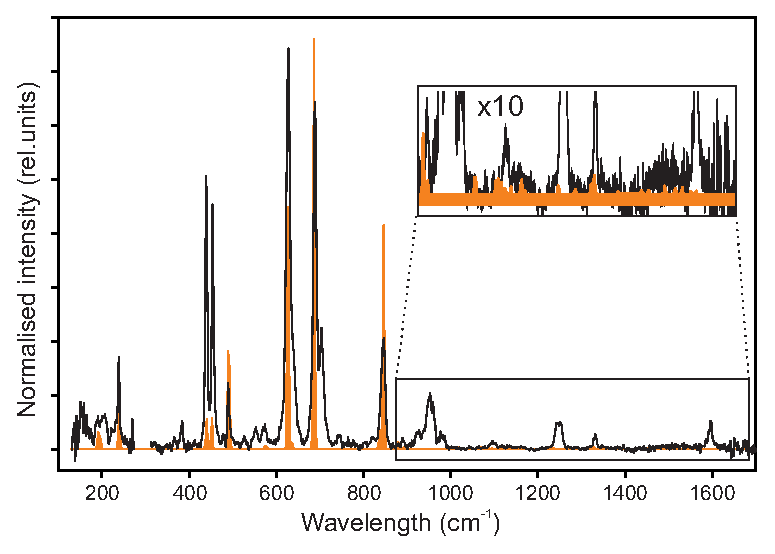
\includegraphics{chapters/HC3N+/overlay_FIT_pred.eps}
    \caption{Bending region of the IRPD spectrum of \neion\ (black) overlaid with the bands predicted from the fitted spectroscopic parameters (orange). For the assignment of weaker
    features please see Table \ref{tab:bend-freqs}. A zoom of the $900-1600$~\wn region is presented to show the large density of transitions of weak intensity.}
    \label{fig:FIT_overlay}
\end{figure*}


\subsection{Influence of the rare-gas tag}
\label{sec:ne-att}
One of the main disadvantages of the IRPD method is that the RG-ion complex is taken as a proxy for the spectrum of the bare ion. 
For larger, closed-shell molecular ions the attachment or rare-gas atoms like Ne or He typically only results in minimal shifts of the vibrational frequencies \cite{Marimuthu2020LaboratorySpectroscopy, Marimuthu2021InfraredCH3CNH+, Thorwirth2020Molecular+, Jasik2013, Douberly2008}, but symmetry-breaking effects were observed, e.g., in the case of cyclic C$_3$H$_3^+$ \cite{Dopfer2002InfraredIsomers, Botschwina2011}.
The influence of the tag on the bending modes of RT-affected open-shell species has, however, not yet been investigated. 
When comparing the observed splitting pattern of the \neion\ to that of the earlier ZEKE work \cite{Dai2015TheCalculations} of the bare \ion\ we note two key differences: First, due to the different selection rules we have on the one hand recorded several features that have not been observed previously, such as the 6$^1\Delta_{5/2}$ fundamental, but on the other, we failed to see several combination bands and overtones, such as the bands at 1414 and 1460 \wn\ (see Appendix Table \ref{tab:bend-freq-dai} for a full comparison between the bands observed with ZEKE \cite{Dai2015TheCalculations} and IRPD). 
Secondly, we only see one of the two SO components since the ions are cooled down to their vibrational and SO ground state ($\Pi_{3/2}$) and the selection rule $\Delta P = \pm 1$ for the bending modes must be obeyed.
Finally, some of the bands that were observed by both methods are shifted compared to each other.
To capture this effect in a reliable way the fitted spectroscopic parameters that were presented before in Table \ref{tab:par} were compared. 
Even though the parameters agree fairly well, the largest deviation is seen in the RT constant of mode $\nu_5$ ($\epsilon_5$), which represents the C-C-H bending.
We hypothesize that this discrepancy is a result of the Ne attachment.

To investigate the influence of the Ne attachment a scan of the \neion\ potential energy surface was made. 
The Ne atom was attached to the middle C-atom of the \ion\ and moved around the ion, with all geometry parameters relaxed except for the angle $\Theta$, see inlay in Fig. \ref{fig:PES_Ne-ion}.
For all \neion geo-metries the bare ion remained linear so that a symmetry plane for the Ne-ion
complex could be defined (here xz). The wavefunction can then be either symmetric, A’, or
asymmetric, A”, with regard to this plane, where the $\Pi_x$ orbital is partially filled for the A’ state and
completely filled for the A” state. 

Figure \ref{fig:PES_Ne-ion} shows the calculated counter-poise corrected interaction energy
as a function of the Ne angle for both A’ and A” symmetry. For both symmetries, the global
minimum is located at $\Theta=180^{\circ}$, which represents linear attachment of the Ne on the H atom,
though both states show fairly different potential energy surfaces. Generally, the A’ state is lower
in energy than the A” state, which is likely due to the lower electron density in the xz-plane for A’
compared to A”. In order to explain the shape of the curves we can look at the Mulliken charges
of the bare \ion. The charges on the H, C1, C2, C3, N are +0.37, +0.02, +0.61, +0.09 and
-0.08, respectively. Since the binding strength with the Ne is mainly determined by electrostatic
interaction the binding will be stronger for a more positive charge. Furthermore, electrostatic
repulsion of the $\Pi_x$ orbital must be taken into account. For the A” state this orbital is completely
filled so that we only see minima at the H ($\Theta=180^{\circ}$) and C2 $\Theta=80^{\circ}$ positions, where the
positive charge is largest. For the A’ the $\Pi_x$ orbital is only partially filled, lowering the electrostatic
repulsion and allowing the Ne to come closer to the ion thus increasing its interaction energy. For
this state a second minimum can then be distinguished at a bent geometry, with $\Theta=120^{\circ}$ and a
$\sim$ 40 \wns barrier to linearity.

Since the Ne atom attaches on the H atom we expect the largest impact to be on the modes that involve this hydrogen, so the C-H stretch ($\nu_1$) and the C-C-H bend ($\nu_5$). Harmonic wavenumber calculations (see Table \ref{tab:Ne-attach}) indeed show that these modes are most affected.
Here modes $\nu1-\nu7$ correspond to the vibrations of the bare ion, $\nu_8$ to the Ne-H stretch
and $\nu_9$ to the Ne-H bending. The fact that the bending modes $\nu_9$ are not fully degenerate indicates
that also this mode is Renner-Teller affected and may couple to the bending modes of the bare
\ion. Whereas in the IRPD experiment the C-H stretching wavenumber is about 60~\wns blue-shifted, harmonic wavenumber calculations actually predict a redshift. We hypothesize that this blue shift could be a result of a restriction of the H-stretching amplitude due to the Ne attachment and a subsequent reduction of the anharmonicity of this mode, resulting in a relative blue-shift. Regarding the C-H bending mode, it is beyond the scope of this study to calculate the effect of the Ne attachment on the vibronic splitting patterns: In principle the attachment leads to a six-atom linear open-shell species, introducing an additional degenerate bending mode which likely interacts with the three bending modes of the bare ion discussed above, and is expected to show large-amplitude vibrational characteristics. However, the calculated position of the Ne attachment could explain the relatively large deviation of the RT constant of mode $\nu_5$ with respect to the earlier PES work.

\begin{figure}
    \centering
    % 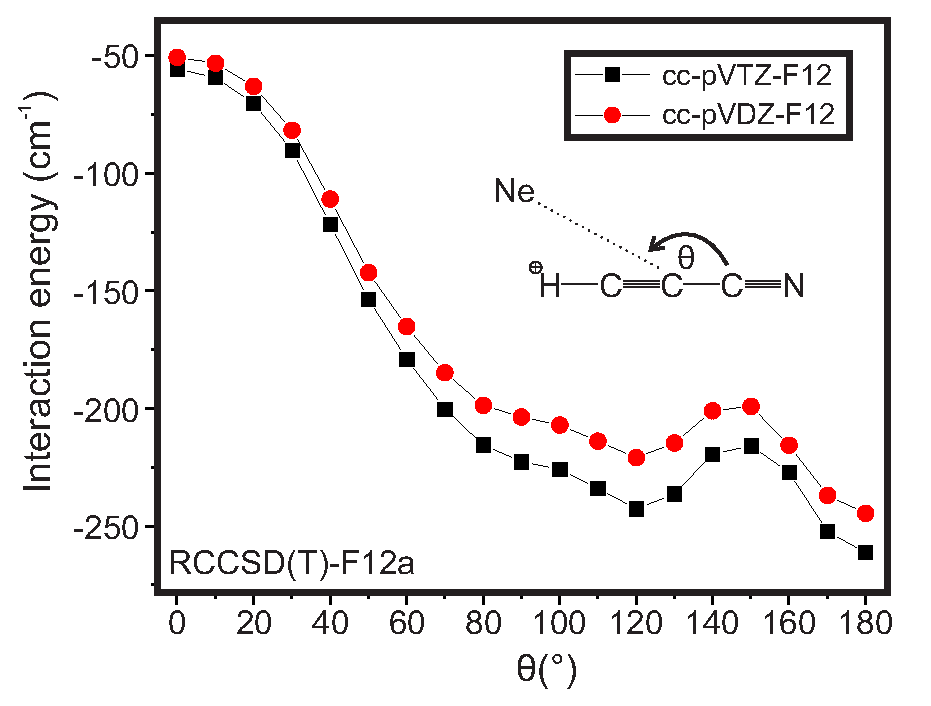
\includegraphics[width=1\textwidth]{chapters/HC3N+/PES_Ne-HC3N+.eps}
    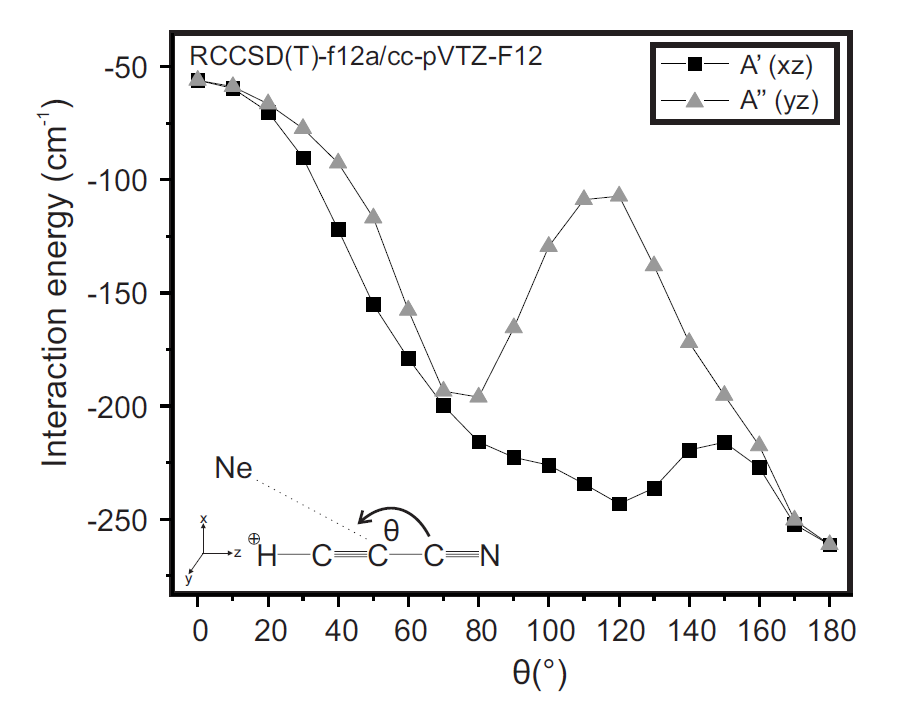
\includegraphics[width=1\textwidth]{chapters/HC3N+/figures/PES_HC3N+_Ne_VTZ_A1_A2.png}
    \caption{Calculated interaction energy as a function of the Ne angle with respect to the molecular axis. A’ represents the symmetric electronic wavefunction, where the $\Pi_x$ orbitals are partially
    filled. A” represents the antisymmetric electronic wavefunction, where the $\Pi_x$ orbitals are
    completely filled}
    \label{fig:PES_Ne-ion}
\end{figure}

\begin{table}
\caption{\label{tab:Ne-attach} Harmonic vibrational frequencies of \ion and \neion\ calculated on RCCSD(T)-F12a/cc-pVTZ-F12 level of theory.}
\begin{threeparttable}
% \begin{ruledtabular}
    \footnotesize
    \begin{tabular}{l c c c c c c c c c c}
      & $\nu_1$ & $\nu_2$ & $\nu_3$ & $\nu_4$  & $\nu_5$ \tnote{1} & $\nu_6$\tnote{1} & $\nu_7$ \tnote{1} & $\nu_8$ & $\nu_9$ \tnote{1} \\
     \hline
    \ion& 3317 & 2222 & 1868 & 908 & [771,644] & [461,445] & [196,187] & $\ldots$ & $\ldots$\\
    \neion& 3306 & 2221 & 1869 & 910 & [785,662] & [463,447] & [203,196] & 68 & [28,26]
    \end{tabular}
    % \end{ruledtabular}
    \begin{tablenotes}
    \item[1] The $x$- and $y$- components of the bending frequencies are given between brackets
    \end{tablenotes}
    \end{threeparttable}
\end{table}


\section{Conclusions}

In this work, we have investigated the vibrational structure of the \ion\ ion with
IRPD. The combination of a cryogenic ion trap with the wide wavenumber coverage of the FEL-1 and FEL-2 free electron lasers allowed to probe the low-lying RT disturbed bending modes directly, giving complementary information to earlier PES work \cite{Dai2015TheCalculations}. The obtained spectrum was fitted with an effective Hamiltonian and the resulting spectroscopic parameters are in reasonable agreement with the \emph{ab initio} and experimental data of \citet{Dai2015TheCalculations}. The largest deviations were found in the parameters describing the \chemfig{H-C~C} bending mode $\nu_5$, which has the largest RT coupling of the three bending modes. We hypothesize that this discrepancy is a direct result of the Ne attachment, which was calculated to bind linearly on the H atom. This hypothesis is strengthened by the large blue shift (60 \wn) we observe for the \chemfig{C-H} ($\nu_1$) stretching mode compared to the other stretches.

This relatively large impact of the Ne on the \ion\ raises the question of whether the IRPD method may be suitable to investigate these RT-affected ions, but currently, no alternative tag-free methods are available. To overcome the problems of the rare-gas attachment one might look into a way to elucidate the rare-gas effect on these complex open-shell species systematically by using different rare-gas tags (e.g. Ar, or N$_2$) or attaching multiple tags to the same ion. This would not only help to extrapolate to the bare-ion spectrum but also gives insight into weakly-bound system interactions. Furthermore, this data might act as a theory benchmark for future research combining the large-amplitude motion of the tag with the vibronic coupling effects of the ion.
